% Compile with latex, then dvisvgm --no-fonts --exact --bbox=papersize.
\documentclass[tikz,border=8pt]{standalone}
\usepackage[T1]{fontenc}
\usepackage{lmodern}
\begin{document}
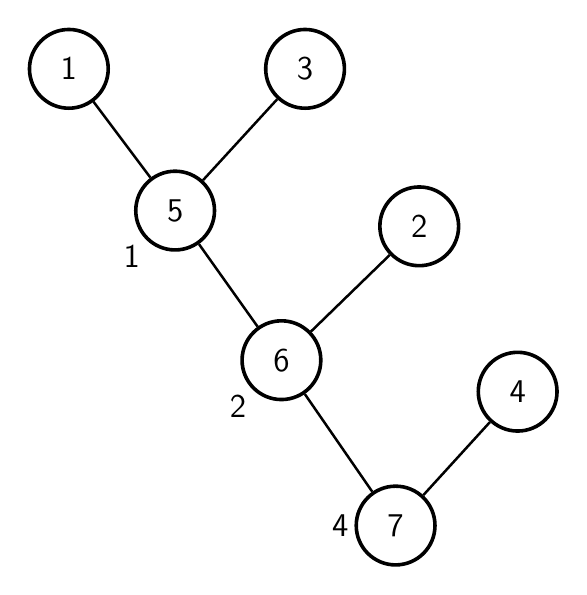
\begin{tikzpicture}[
    font=\sffamily\large,
    vertex/.style={circle,draw,line width=1.3pt,fill=white,
                   minimum size=10mm,inner sep=0pt},
    edge/.style={line width=0.9pt},
    weight/.style={font=\sffamily\large,inner sep=2pt}]
  % Node numbers are inside circles; merge weights are outside to the left.
  % Merge {1,3} at weight 1, then add 2 at weight 2, then 4 at weight 4.
  \node[vertex] (1) at (0,0) {1};
  \node[vertex] (3) at (3,0) {3};
  \node[vertex,label={[weight]below left:1}] (5) at (1.35,-1.8) {5};
  \node[vertex] (2) at (4.45,-2) {2};
  \node[vertex,label={[weight]below left:2}] (6) at (2.7,-3.7) {6};
  \node[vertex] (4) at (5.7,-4.1) {4};
  \node[vertex,label={[weight]left:4}] (7) at (4.15,-5.8) {7};
  \draw[edge] (1) -- (5) -- (3);
  \draw[edge] (5) -- (6) -- (2);
  \draw[edge] (6) -- (7) -- (4);
\end{tikzpicture}
\end{document}
